% One-page summary of Experiments 1-2 (+ Tests A, C) and the proposed Test B.
% Every number comes from the saved runs in ../results/ (see ../exp2/LOOP_LOG.md).
% Build: pdflatex noop_onepager.tex
\documentclass[10pt]{article}
\usepackage[letterpaper,margin=0.42in]{geometry}
\usepackage[T1]{fontenc}
\usepackage[scaled=0.92]{helvet}
\renewcommand{\familydefault}{\sfdefault}
\usepackage{microtype}
\usepackage{xcolor}
\usepackage{tikz}
\usetikzlibrary{arrows.meta,positioning,calc,decorations.pathreplacing,shapes.geometric}
\usepackage{enumitem}
\usepackage{booktabs}
\usepackage{amssymb}
\pagestyle{empty}
\setlength{\parindent}{0pt}
\setlength{\parskip}{2pt}
\setlist{nosep,leftmargin=1.1em,itemsep=1pt}

% Validated categorical slots (dataviz reference palette, light) + chart ink
\definecolor{cblue}{HTML}{2A78D6}
\definecolor{corange}{HTML}{EB6834}
\definecolor{caqua}{HTML}{1BAF7A}
\definecolor{cyellow}{HTML}{EDA100}
\definecolor{ink}{HTML}{0B0B0B}
\definecolor{ink2}{HTML}{52514E}
\definecolor{muted}{HTML}{898781}
\definecolor{grid}{HTML}{E1E0D9}
\definecolor{axis}{HTML}{C3C2B7}
\definecolor{plane}{HTML}{F4F3EF}
\color{ink}

\newcommand{\sect}[2]{\par\vspace{5pt}{\color{cblue}\bfseries\small #1}\hspace{0.4em}{\bfseries\small #2}\par\nointerlineskip\vspace{2pt}{\color{axis}\hrule height 0.4pt}\vspace{3pt}}
\newcommand{\tok}[1]{\texttt{\detokenize{#1}}}
\newcommand{\keybox}[1]{\par\vspace{2pt}\fcolorbox{axis}{plane}{\parbox{\dimexpr\linewidth-2\fboxsep-2\fboxrule}{#1}}\par}

\begin{document}
\fontsize{8.8}{10.7}\selectfont

%================ HEADER ================
{\LARGE\bfseries When do GPT-2's attention heads go idle?}\\[1pt]
{\normalsize\color{ink2} From a random-token ``no-op'' baseline to a phrase-sensitive effect, and the circuit test that comes next}\\[1pt]
{\scriptsize\color{muted} Pablo Leyva \,·\, no-op research \,·\, GPT-2 small, TransformerLens + Hugging Face on identical token ids \,·\, October 2026}

\vspace{3pt}
\keybox{\textbf{The question.} At the final token of a sequence, some attention heads do work and others park their attention on the first token (BOS, the ``sink''), which acts as a \emph{no-op}. \textbf{What switches a head into the no-op state?} We feed GPT-2 small a BOS token plus 32 random tokens and measure, for each of the 144 heads, the attention the final token pays to BOS (\emph{sink mass}). Then we change the input in controlled ways and watch which heads park more or less.}

\vspace{2pt}
%================ TWO COLUMNS ================
\noindent
\begin{minipage}[t]{0.488\linewidth}

\sect{1}{Experiment 1: the no-op baseline}
On rare-token noise (ids 1000--39999), \textbf{74\% of heads park on BOS} at the final token, and parking grows with depth:

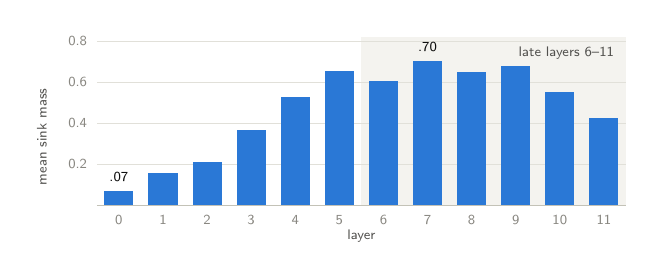
\begin{tikzpicture}[x=0.56cm,y=2.6cm]
  \fill[plane] (5.5,0) rectangle (11.5,0.82);
  \node[font=\tiny,color=ink2,anchor=north east] at (11.45,0.82) {late layers 6--11};
  \foreach \y in {0.2,0.4,0.6,0.8} {
    \draw[grid,line width=0.3pt] (-0.5,\y) -- (11.5,\y);
    \node[font=\tiny,color=muted,anchor=east] at (-0.5,\y) {\y};
  }
  \foreach \v [count=\i from 0] in {0.068,0.156,0.209,0.368,0.528,0.657,0.609,0.704,0.653,0.681,0.555,0.426} {
    \fill[cblue] (\i-0.33,0) rectangle (\i+0.33,\v);
    \node[font=\tiny,color=muted,anchor=north] at (\i,0) {\i};
  }
  \draw[axis,line width=0.5pt] (-0.5,0) -- (11.5,0);
  \node[font=\tiny,color=ink2] at (5.5,-0.15) {layer};
  \node[font=\tiny,color=ink,anchor=south] at (7,0.704) {.70};
  \node[font=\tiny,color=ink,anchor=south] at (0,0.068) {.07};
  \node[font=\tiny,color=ink2,anchor=west,rotate=90] at (-1.75,0.05) {mean sink mass};
\end{tikzpicture}

Rare vs common tokens leave the share of parked heads almost unchanged, but individual heads move in \emph{opposite} directions: late heads work more on rare tokens and park on common ones.

\sect{2}{What moves them (single-token follow-up)}
\begin{itemize}
  \item The late-head shift comes from the \textbf{whole context}, not from the final token alone.
  \item Swapping one context token barely matters, \textbf{except right before the final token}: single-token effects there are about $6\times$ larger than mid-sequence (median per-head spread .029 vs .005).
\end{itemize}

\sect{3}{Experiment 2: write a phrase into the noise}
Each base row is overwritten at positions 29--31; everything else, including the final token, stays the same, so every effect is a within-row difference. A real example row (rare base):

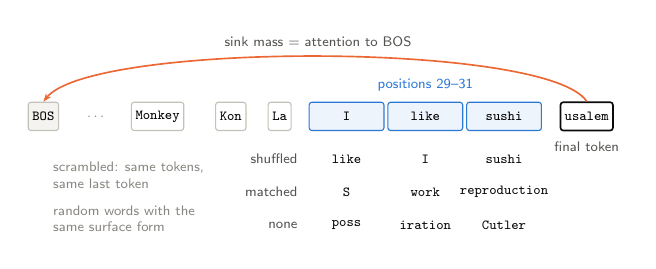
\begin{tikzpicture}[tk/.style={draw=axis,fill=white,rounded corners=1pt,inner sep=1.5pt,minimum height=0.36cm,font=\ttfamily\tiny},
                    sl/.style={tk,draw=cblue,fill=cblue!8,minimum width=0.95cm},
                    lab/.style={font=\tiny,color=ink2,anchor=east}]
  \node[tk,fill=plane] (bos) at (0,0) {BOS};
  \node[font=\tiny,color=muted] at (0.68,0) {\dots};
  \node[tk] (a) at (1.45,0) {\detokenize{ Monkey}};
  \node[tk] (b) at (2.38,0) {\detokenize{ Kon}};
  \node[tk] (c) at (3.0,0) {La};
  \node[sl] (s1) at (3.85,0) {\detokenize{ I}};
  \node[sl] (s2) at (4.85,0) {\detokenize{ like}};
  \node[sl] (s3) at (5.85,0) {\detokenize{ sushi}};
  \node[tk,draw=ink,line width=0.6pt] (q) at (6.9,0) {usalem};
  \node[font=\tiny,color=ink2,anchor=north] at (6.9,-0.2) {final token};
  \node[font=\tiny,color=cblue,anchor=south] at (4.85,0.2) {positions 29--31};
  \draw[-{Stealth[length=3pt]},corange,line width=0.6pt] (q.north) .. controls (6.4,0.95) and (0.6,0.95) .. (bos.north)
       node[pos=0.5,above,font=\tiny,color=ink2] {sink mass = attention to BOS};
  % variants
  \foreach \nm/\x/\y/\z [count=\r] in {shuffled/like/I/sushi, matched/S/work/reproduction, none/poss/iration/Cutler} {
    \node[lab] at (3.35,-0.42*\r-0.12) {\nm};
    \node[font=\ttfamily\tiny,color=ink] at (3.85,-0.42*\r-0.12) {\x};
    \node[font=\ttfamily\tiny,color=ink] at (4.85,-0.42*\r-0.12) {\y};
    \node[font=\ttfamily\tiny,color=ink] at (5.85,-0.42*\r-0.12) {\z};
  }
  \node[font=\tiny,color=muted,anchor=west,align=left] at (0,-0.75) {scrambled: same tokens,\\same last token};
  \node[font=\tiny,color=muted,anchor=west,align=left] at (0,-1.3) {random words with the\\same surface form};
\end{tikzpicture}

\vspace{1pt}
\textbf{Interaction} = (phrase $-$ none) $-$ $\Sigma$ (each word alone $-$ none): what the combination adds beyond its words. Findings over three iterations:
\begin{itemize}
  \item Near the final token, a phrase makes \textbf{layer 6--11 heads park more}; written mid-sequence (positions 14--16) it does little.
  \item The phrase adds sink \textbf{beyond its single words}; the scrambled order adds much less. Single-word effects explain none of the order effect ($r^2 \approx 0$).
  \item \textbf{Not surprisal}: the model's surprise at the phrase explains about a tenth of the order effect, and across phrases the effect does not track it.
\end{itemize}

\end{minipage}\hfill
\begin{minipage}[t]{0.488\linewidth}

\sect{4}{It generalizes: 3 phrase types $\times$ 2 base classes}
Late-layer interaction, mean over 12 phrases per template, 95\% CI over phrases:

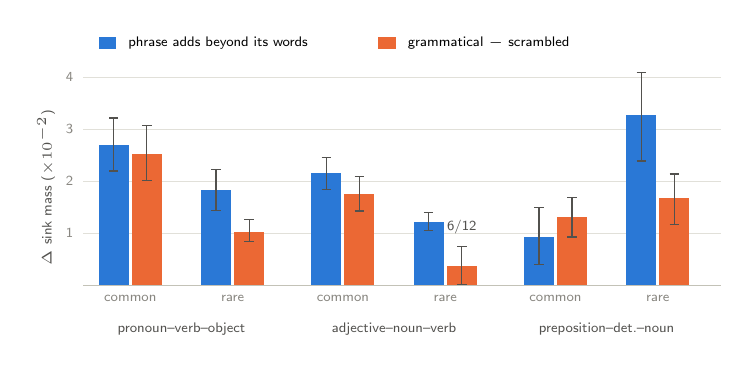
\begin{tikzpicture}[x=1cm,y=0.66cm]
  % legend
  \fill[cblue] (0.05,4.55) rectangle (0.27,4.77); \node[font=\tiny,anchor=west] at (0.3,4.66) {phrase adds beyond its words};
  \fill[corange] (3.6,4.55) rectangle (3.82,4.77); \node[font=\tiny,anchor=west] at (3.85,4.66) {grammatical $-$ scrambled};
  \foreach \y in {1,2,3,4} {
    \draw[grid,line width=0.3pt] (-0.15,\y) -- (7.95,\y);
    \node[font=\tiny,color=muted,anchor=east] at (-0.15,\y) {\y};
  }
  % group: x, nl, nl_lo, nl_hi, ord, ord_lo, ord_hi, base label
  \foreach \x/\a/\al/\ah/\b/\bl/\bh/\lab in {
      0.45/2.70/2.20/3.22/2.52/2.01/3.07/common, 1.75/1.83/1.44/2.23/1.03/0.84/1.27/rare,
      3.15/2.16/1.84/2.46/1.76/1.43/2.09/common, 4.45/1.22/1.05/1.40/0.37/0.02/0.74/rare,
      5.85/0.93/0.40/1.49/1.31/0.93/1.69/common, 7.15/3.27/2.39/4.09/1.68/1.17/2.14/rare} {
    \fill[cblue] (\x-0.40,0) rectangle (\x-0.02,\a);
    \fill[corange] (\x+0.02,0) rectangle (\x+0.40,\b);
    \draw[ink2,line width=0.45pt] (\x-0.21,\al) -- (\x-0.21,\ah) (\x-0.27,\al) -- (\x-0.15,\al) (\x-0.27,\ah) -- (\x-0.15,\ah);
    \draw[ink2,line width=0.45pt] (\x+0.21,\bl) -- (\x+0.21,\bh) (\x+0.15,\bl) -- (\x+0.27,\bl) (\x+0.15,\bh) -- (\x+0.27,\bh);
    \node[font=\tiny,color=muted,anchor=north] at (\x,0) {\lab};
  }
  \draw[axis,line width=0.5pt] (-0.15,0) -- (7.95,0);
  \node[font=\tiny,color=ink2] at (1.1,-0.85) {pronoun--verb--object};
  \node[font=\tiny,color=ink2] at (3.8,-0.85) {adjective--noun--verb};
  \node[font=\tiny,color=ink2] at (6.5,-0.85) {preposition--det.--noun};
  \node[font=\tiny,color=ink2,anchor=south] at (4.66,0.80) {6/12};
  \node[font=\tiny,color=ink2,anchor=west,rotate=90] at (-0.62,0.2) {$\Delta$ sink mass ($\times 10^{-2}$)};
\end{tikzpicture}

Both effects are positive in all six cells. The weak spot: for adjective phrases on rare bases, the order effect holds in only 6 of 12 phrases. Which base class shows more depends on the template, and we can't yet explain why.

\sect{5}{Test A: the work is done by adjacent word pairs}
The phrase's interaction splits exactly into word pairs plus a three-word term (share of the total):

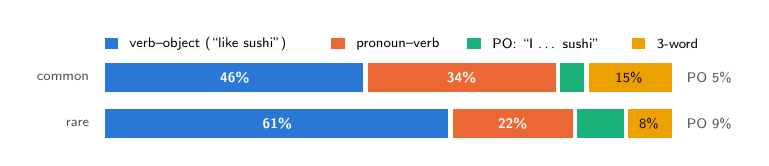
\begin{tikzpicture}[x=0.072cm,y=0.58cm]
  \foreach \lab/\yy/\vo/\pv/\po/\tr in {common/1/46/34/5/15, rare/0/61/22/9/8} {
    \node[font=\tiny,color=ink2,anchor=east] at (-1,\yy) {\lab};
    \fill[cblue]   (0,\yy-0.32) rectangle (\vo-0.4,\yy+0.32);
    \fill[corange] (\vo+0.4,\yy-0.32) rectangle (\vo+\pv-0.4,\yy+0.32);
    \fill[caqua]   (\vo+\pv+0.4,\yy-0.32) rectangle (\vo+\pv+\po-0.4,\yy+0.32);
    \fill[cyellow] (\vo+\pv+\po+0.4,\yy-0.32) rectangle (100,\yy+0.32);
    \node[font=\tiny\bfseries,color=white] at (\vo/2,\yy) {\vo\%};
    \node[font=\tiny\bfseries,color=white] at (\vo+\pv/2,\yy) {\pv\%};
    \node[font=\tiny,color=ink] at (\vo+\pv+\po+\tr/2,\yy) {\tr\%};
    \node[font=\tiny,color=ink2,anchor=west] at (101,\yy) {PO \po\%};
  }
  \fill[cblue] (0,1.62) rectangle (2.4,1.86); \node[font=\tiny,anchor=west] at (2.7,1.74) {verb--object (``like sushi'')};
  \fill[corange] (40,1.62) rectangle (42.4,1.86); \node[font=\tiny,anchor=west] at (42.7,1.74) {pronoun--verb};
  \fill[caqua] (64,1.62) rectangle (66.4,1.86); \node[font=\tiny,anchor=west] at (66.7,1.74) {PO: ``I \dots\ sushi''};
  \fill[cyellow] (93,1.62) rectangle (95.4,1.86); \node[font=\tiny,anchor=west] at (95.7,1.74) {3-word};
\end{tikzpicture}

The pair \textbf{ending right before the final token} carries about half; the non-adjacent pair and the three-word term add little.

\sect{6}{How much to trust it}
\begin{itemize}
  \item \textbf{35 of 43 pre-registered predictions held.} The misses were real surprises: word order mattered more than predicted, mid-sequence placement was not a full no-op, verb--object carried 46\% (predicted $\ge$ 50\%), the adjective/rare cell above, plus two hairline sanity misses.
  \item TransformerLens and Hugging Face agree to $<10^{-4}$ on every run. The no-phrase rows reproduce Experiment 1 ($r \ge 0.9993$), re-runs are bit-identical, and the random-word placebo flags at most 0.3\% of tests in any run.
  \item Limits: GPT-2 small only, 3 hand-picked templates, and small effects (+0.01 to +0.03 mean sink mass over the late heads).
\end{itemize}

\end{minipage}

%================ BOTTOM BAND ================
\vspace{3pt}
\keybox{%
\begin{minipage}[c]{0.355\linewidth}
\raggedright
\textbf{Working hypothesis.} Late heads park on BOS (go no-op) when the words right before the final token form a \textbf{coherent adjacent pair}. Open question: is that no-op \emph{computed} by a circuit, or a passive fallback?

\vspace{3pt}
{\color{cblue}\bfseries Next: Test B, find the circuit}\\
{\color{muted}\scriptsize design and predictions: \texttt{exp2/testb.md}}\\[1pt]
Compare ``verb + object'' (\tok{like sushi}) with ``object alone'': the runs differ only at position 30. Patch activations from one run into the other:
\begin{enumerate}[label=\arabic*.,leftmargin=1.2em]
  \item residual stream by position $\times$ layer: where does the signal live?
  \item query vs key of the late heads: does the final token ask differently, or do the phrase tokens look different?
  \item single early-head outputs: who writes it?
  \item switch those heads off: does the extra parking disappear?
\end{enumerate}
\end{minipage}\hfill
\begin{minipage}[c]{0.28\linewidth}
\centering
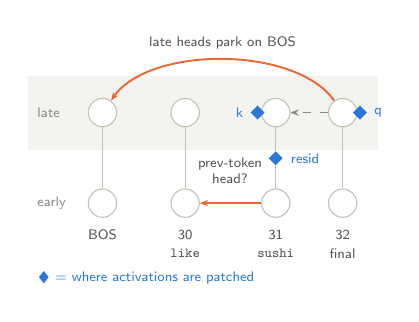
\begin{tikzpicture}[x=1cm,y=1cm,
    nd/.style={circle,draw=axis,fill=white,inner sep=0pt,minimum size=0.36cm},
    pt/.style={diamond,fill=cblue,inner sep=1.3pt}]
  \fill[plane] (-0.1,0.68) rectangle (4.35,1.62);
  \node[font=\tiny,color=muted,anchor=west] at (-0.1,1.15) {late};
  \node[font=\tiny,color=muted,anchor=west] at (-0.1,0.0) {early};
  \foreach \nm/\x in {BOS/0.85, 30/1.9, 31/3.05, 32/3.9} {
    \node[nd] (e\nm) at (\x,0) {};
    \node[nd] (l\nm) at (\x,1.15) {};
    \draw[axis,line width=0.4pt] (e\nm) -- (l\nm);
    \node[font=\tiny,color=ink2,anchor=north] at (\x,-0.22) {\nm};
  }
  \node[font=\ttfamily\tiny,color=ink2,anchor=north] at (1.9,-0.46) {\detokenize{ like}};
  \node[font=\ttfamily\tiny,color=ink2,anchor=north] at (3.05,-0.46) {\detokenize{ sushi}};
  \node[font=\tiny,color=ink2,anchor=north] at (3.9,-0.46) {final};
  \draw[-{Stealth[length=3pt]},corange,line width=0.7pt] (e31) -- (e30);
  \node[font=\tiny,color=ink2,anchor=south,align=center] at (2.47,0.12) {prev-token\\head?};
  \draw[-{Stealth[length=3pt]},corange,line width=0.7pt] (l32) .. controls (3.3,2.0) and (1.45,2.0) .. (lBOS)
       node[pos=0.5,above,font=\tiny,color=ink2] {late heads park on BOS};
  \draw[-{Stealth[length=3pt]},muted,dashed,line width=0.5pt] (l32) -- (l31);
  \node[pt] at (3.05,0.57) {}; \node[font=\tiny,color=cblue,anchor=west] at (3.12,0.57) {resid};
  \node[pt] at (4.12,1.15) {}; \node[font=\tiny,color=cblue,anchor=west] at (4.18,1.15) {q};
  \node[pt] at (2.82,1.15) {}; \node[font=\tiny,color=cblue,anchor=east] at (2.76,1.15) {k};
  \node[font=\tiny,color=cblue,anchor=north west] at (-0.1,-0.75) {$\blacklozenge$ = where activations are patched};
\end{tikzpicture}
\end{minipage}\hfill
\begin{minipage}[c]{0.325\linewidth}
\textbf{Pre-registered predictions}
\begin{itemize}
  \item[B1] The signal moves from position 30 to 31 in early layers (31 recovers $\ge$ 50\% from layer 4 on).
  \item[B2] Key side: patching the late heads' keys at 30--31 recovers more than their query at 32.
  \item[B3] The top writers include a known previous-token head (e.g.\ L4H11, L2H2).
  \item[B4] Switching off the top 3 writers removes $\ge$ 50\% of the effect; 3 random heads $<$ 20\%.
\end{itemize}
\vspace{2pt}
\textbf{Why it matters.} It decides whether the no-op is computed or a fallback, whether heads ``find nothing to read'' or ``stop asking'', and it gives Experiment 3 heads to switch off or patch in.
\end{minipage}}

\end{document}
